\chapter{對易可觀測量、能量相位與自旋進動}

\lectureoverview{我們先從不確定性的定性意義談起。兩個可觀測量只有在具有一組完備的共同本徵基時，才能同時具有確定值；這等價於它們的算符彼此對易。接著我們回顧酉演化與Schr\"odinger方程，比較對易子與經典卜瓦松括號，在能量基底中求解含時方程，並將結果應用於磁場中的自旋。最後的計算將得到自旋期望值的進動、一般自旋哈密頓量的兩個能階，以及側向期望值與能隙一半能量的光子之間的區別。}

二態自旋仍是最簡單的量子系統。三態希爾伯特空間是下一個最簡單的抽象可能性；兩個自旋則已有四個彼此正交的基底態。我們暫時還不把兩個自旋組合起來，雖然這一步已經不遠，而且會帶來糾纏。首先，我們應完成單一自旋的問題，並更扎實地建立不確定性與時間演化的概念。

\section{兩個量何時能同時具有確定值}

好的測量應該可以重複。如果測量某個可觀測量得到數值\(l\)，緊接著再測一次應該會得到相同數值。因此，第一次測量必須使系統至少暫時處於相應算符的本徵態：
\begin{equation}
L\ket{l}=l\ket{l}.
\end{equation}
這項操作上的陳述，已足以揭示不確定性的定性起源。

假設兩個可觀測量\(L\)與\(M\)可以同時測量。聯合測量必須使回報的兩個數值都確定。因此，測量後可能出現的狀態必須是兩個算符的共同本徵向量。在此處討論的有限維情形中，我們可以選取一組完備的正交歸一集合\(\{\ket{i}\}\)，使其滿足
\begin{equation}
L\ket{i}=l_i\ket{i},
\qquad
M\ket{i}=m_i\ket{i}.
\label{eq:l5-common-eigenvectors}
\end{equation}

\begin{remark}
此處的「\emph{基底}」指完備的正交歸一基底。線性代數也允許非正交基底，但正交歸一的慣例對量子態特別自然。若本徵值簡併，則本徵空間內仍有選擇自由；我們可以在該空間中選取正交歸一的本徵向量。
\end{remark}

\begin{theorem}
兩個有限維厄米可觀測量能同時測量，若且唯若它們有一組完備的共同本徵基底；這也等價於兩者對易。
\end{theorem}

由式~\eqref{eq:l5-common-eigenvectors}可立即得到正向推論。先後以一種順序作用，得到
\begin{align}
ML\ket{i}
&=M\bigl(l_i\ket{i}\bigr)\\
&=l_i m_i\ket{i},
\end{align}
若反過來作用，則得到
\begin{align}
LM\ket{i}
&=L\bigl(m_i\ket{i}\bigr)\\
&=m_i l_i\ket{i}.
\end{align}
本徵值是一般的數，因此\(l_i m_i=m_i l_i\)。於是，\(ML\)與\(LM\)對基底中的每個向量作用相同，也就對每個狀態作用相同：
\begin{equation}
[L,M]\equiv LM-ML=0.
\label{eq:l5-commuting-condition}
\end{equation}

\begin{figure}[htbp]
\centering
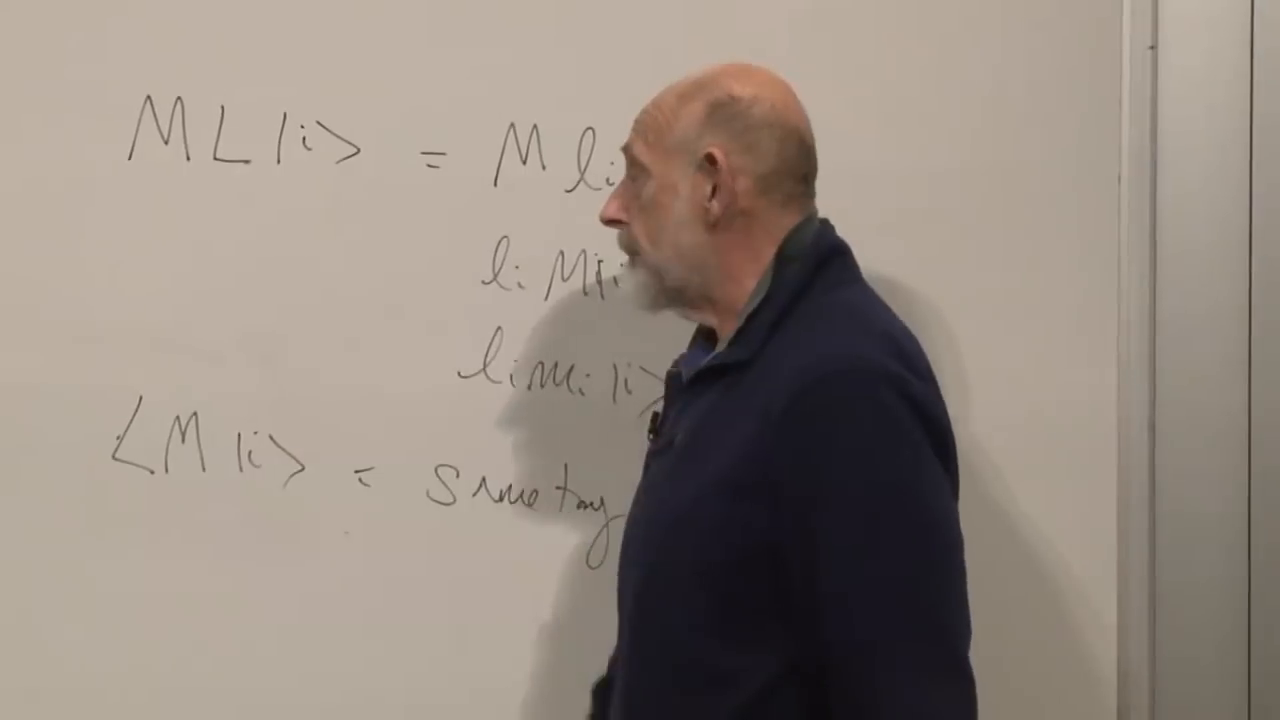
\includegraphics[width=0.86\textwidth]{lecture_05_figure_02.png}
\caption{共同本徵向量的論證導出\(LM-ML=[L,M]=0\)。}
\lectureframe{00:10:30}
\end{figure}

逆向命題也成立：彼此對易的厄米算符可以同時對角化。如果其中一個算符有簡併本徵空間，另一個算符會將該本徵空間映回自身，並可在其中對角化。在每個本徵空間中重複這個步驟，就能得到一組完備的共同本徵基底。

泡利算符提供了第一個重要的反例。\(\sigma_x,\sigma_y,\sigma_z\)中任意兩個算符都不對易。\(\sigma_z\)的本徵態是自旋向上與向下，\(\sigma_x\)的本徵態則是向右與向左。可以將其中一個分量製備成確定值，並重複測量；但無法同時將兩個分量都製備成確定值。這就是尚未引入任何數值不等式之前的不確定性。

稍後我們會定量說明，兩個不對易可觀測量的不確定性如何彼此制約。這裡尚未證明任何數值形式的不確定性原理。目前要說的是比不等式更基本的一點：不對易性使狀態無法同時為兩個量指定確定值。

\begin{classroomqa}
\audiencequestion{為什麼同時測量需要共同本徵向量？}
\lecturerresponse{可重複的測量會使測量值在狀態中確定，也就是說，該狀態是被測算符的本徵態。如果同時得到兩個數值，而且兩者都能重複測得，那麼測量後的狀態必須是兩個算符的本徵態。因此，所有可能的聯合測量結果會構成一組共同本徵基底。}
\end{classroomqa}

\begin{classroomqa}
\audiencequestion{這一定涉及兩個不同的粒子嗎？}
\lecturerresponse{不一定，因為\(\sigma_x\)與\(\sigma_z\)本來就作用在同一個自旋上。不過，對於兩個不同的子系統，作用在不同因子上的可觀測量確實會彼此對易：\(A\otimes I\)與\(I\otimes B\)對易。因此，一個自旋的某個分量可以和另一個自旋的某個分量一起測量。稍後我們會看到，組合這類系統會導致糾纏。}
\end{classroomqa}

\section{酉演化及其生成元}

量子力學花了比經典力學長得多的時間才確立狀態的定義，但一旦狀態空間確立，運動規則就相當簡潔。令
\begin{equation}
\ket{\psi(t)}=U(t)\ket{\psi(0)}.
\label{eq:l5-propagator}
\end{equation}
時間演化必須保持狀態的可區辨性；更強地說，它會保持所有內積。對於一組正交歸一基底，
\begin{equation}
\bra{j}U^\dagger(t)U(t)\ket{i}=\delta_{ji},
\end{equation}
因此
\begin{equation}
U^\dagger(t)U(t)=I.
\label{eq:l5-unitarity}
\end{equation}
演化算符是酉算符。

經過零時間時，\(U(0)=I\)。由連續性可知，經過一小段時間\(\epsilon\)的演化，只會與單位算符略有不同。在\(\hbar=1\)的單位制下，寫成
\begin{equation}
U(\epsilon)=I-i\epsilon H+O(\epsilon^2),
\qquad
U^\dagger(\epsilon)=I+i\epsilon H^\dagger+O(\epsilon^2).
\end{equation}
將它代入方程~\eqref{eq:l5-unitarity}，得到
\begin{equation}
H^\dagger=H.
\end{equation}
時間演化的生成元是厄米算符，因此也是可觀測量。它就是哈密頓量。

將無窮小傳播算符作用於狀態，得到
\begin{equation}
\ket{\psi(\epsilon)}
=\ket{\psi(0)}-i\epsilon H\ket{\psi(0)}+O(\epsilon^2).
\end{equation}
重新整理後，便得到黑板上所示的差商：
\begin{equation}
\frac{\ket{\psi(\epsilon)}-\ket{\psi(0)}}{\epsilon}
=-iH\ket{\psi(0)}+O(\epsilon).
\end{equation}

\begin{figure}[htbp]
\centering
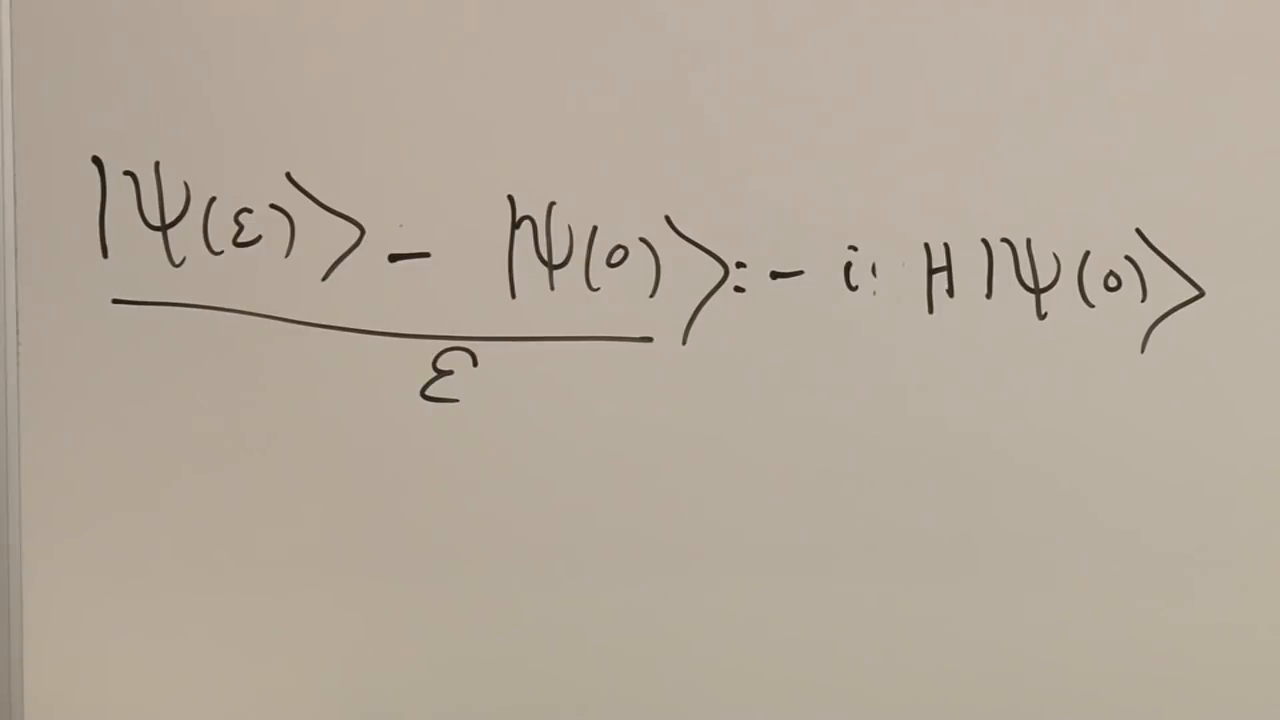
\includegraphics[width=0.86\textwidth]{lecture_05_figure_03.png}
\caption{以差商表示的無窮小演化更新。}
\lectureframe{00:23:33}
\end{figure}

令\(\epsilon\to0\)，便得到含時Schr\"odinger方程：
\begin{equation}
\frac{d}{dt}\ket{\psi(t)}=-iH\ket{\psi(t)}.
\label{eq:l5-schrodinger}
\end{equation}
恢復常數後，即為\(i\hbar\,d\ket{\psi}/dt=H\ket{\psi}\)。

Schr\"odinger最初提出的方程描述的是運動粒子的波函數。上面的算符形式過去稱為廣義Schr\"odinger方程，因為它同樣適用於自旋、三態系統、兩個自旋，乃至任意複雜的系統。如今這個形容詞大多已省略；這就是該方程的一般形式。

方程~\eqref{eq:l5-schrodinger}描述系統在未受擾動時的確定演化。但這不表示每個實驗結果都是確定的。量子態決定各種可能測量結果的機率，而該方程透過振幅的變化來演化這些機率。測量通常會改變狀態，並中斷這種孤立演化。

\begin{classroomqa}
\audiencequestion{每次測量都會擾動系統嗎？}
\lecturerresponse{一般而言會，但有一個重要的例外。如果狀態已經是該可觀測量的本徵態，理想且可重複的測量便能確認其數值而不改變狀態。一般情況下，無法在測量任意可觀測量時，完全不擾動其他與它不相容的性質。}
\end{classroomqa}

\section{能量與定態方程}

由於\(H\)是厄米算符，其本徵值皆為實數，而且本徵向量可以選成一組完備的正交歸一基底：
\begin{equation}
H\ket{E_i}=E_i\ket{E_i}.
\label{eq:l5-time-independent}
\end{equation}
這是Schr\"odinger方程的定態形式。它不是運動方程，而是一個本徵值問題：它要找出系統可能具有的能量值，以及哪些狀態具有確定的能量值。

能譜取決於系統。束縛原子的運動與諧振子都有可數的能階。未受束縛的粒子則可能具有連續能譜。能量可以用許多方式測量；原則上，即使是足夠精確的質量測量，也能透過\(E=mc^2\)得知能量，雖然這很少是實際採用的方法。真實系統本身已有其哈密頓量；物理學家並不指定它，而是設法找出它。一旦知道這個算符，求出它的本徵值與本徵向量就是數學上的工作。

在\(H\)中加上常數\(cI\)，會使每個能量都平移\(c\)。這會讓整個狀態乘上一個共同相位\(e^{-ict}\)，但不會改變機率或期望值。只有能量差會影響此處討論的動力學。

\section{期望值如何演化}

「\emph{期望值}」是統計平均的慣用說法。對可觀測量\(L\)而言，
\begin{equation}
\expect{L}(t)=\bra{\psi(t)}L\ket{\psi(t)}.
\end{equation}
目前只有態向量帶有時間依賴性。對等式兩邊微分，並使用方程~\eqref{eq:l5-schrodinger}及其厄米共軛，
\begin{equation}
\frac{d}{dt}\ket{\psi}=-iH\ket{\psi},
\qquad
\frac{d}{dt}\bra{\psi}=i\bra{\psi}H,
\end{equation}
可得
\begin{align}
\frac{d}{dt}\expect{L}
&=i\bra{\psi}HL\ket{\psi}
  -i\bra{\psi}LH\ket{\psi}\\
&=-i\expect{[L,H]}.
\label{eq:l5-expectation-motion}
\end{align}

\begin{figure}[htbp]
\centering
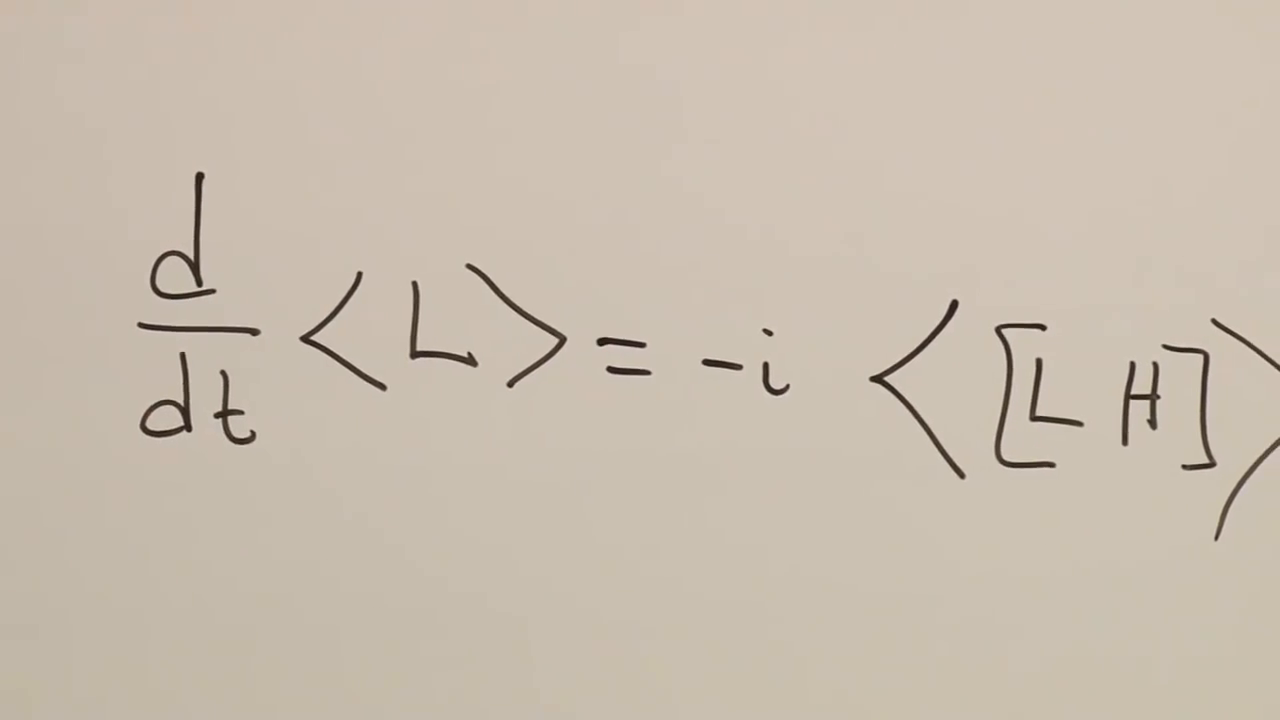
\includegraphics[width=0.86\textwidth]{lecture_05_figure_04.png}
\caption{以對易子表示的期望值運動方程。}
\lectureframe{00:35:35}
\end{figure}

因子\(i\)不會使\(\expect{L}\)變成非實數。對於厄米算符\(L\)與\(H\)，對易子是反厄米算符：
\begin{equation}
[L,H]^\dagger=-[L,H].
\end{equation}
因此，它的期望值純為虛數；乘上\(-i\)後，導數便是實數。

有時會使用以下簡寫：
\begin{equation}
\dot L=-i[L,H].
\end{equation}
此處應將它視為方程~\eqref{eq:l5-expectation-motion}的簡寫，也就是描述平均值的方程。稍後才會介紹讓算符本身帶有時間依賴性的完整表象變換。

\subsection{對易子的代數}

對易子具有反對稱性：
\begin{equation}
[A,B]=-[B,A].
\end{equation}
它們也遵循乘法法則，類似微分的萊布尼茲法則：
\begin{equation}
[AB,C]=A[B,C]+[A,C]B.
\label{eq:l5-product-rule}
\end{equation}
驗證時，須維持每個因子的次序：
\begin{align}
A[B,C]+[A,C]B
&=A(BC-CB)\\
&\quad +(AC-CA)B\\
&=ABC-ACB\\
&\quad +ACB-CAB\\
&=ABC-CAB\\
&=[AB,C].
\end{align}

\begin{figure}[htbp]
\centering
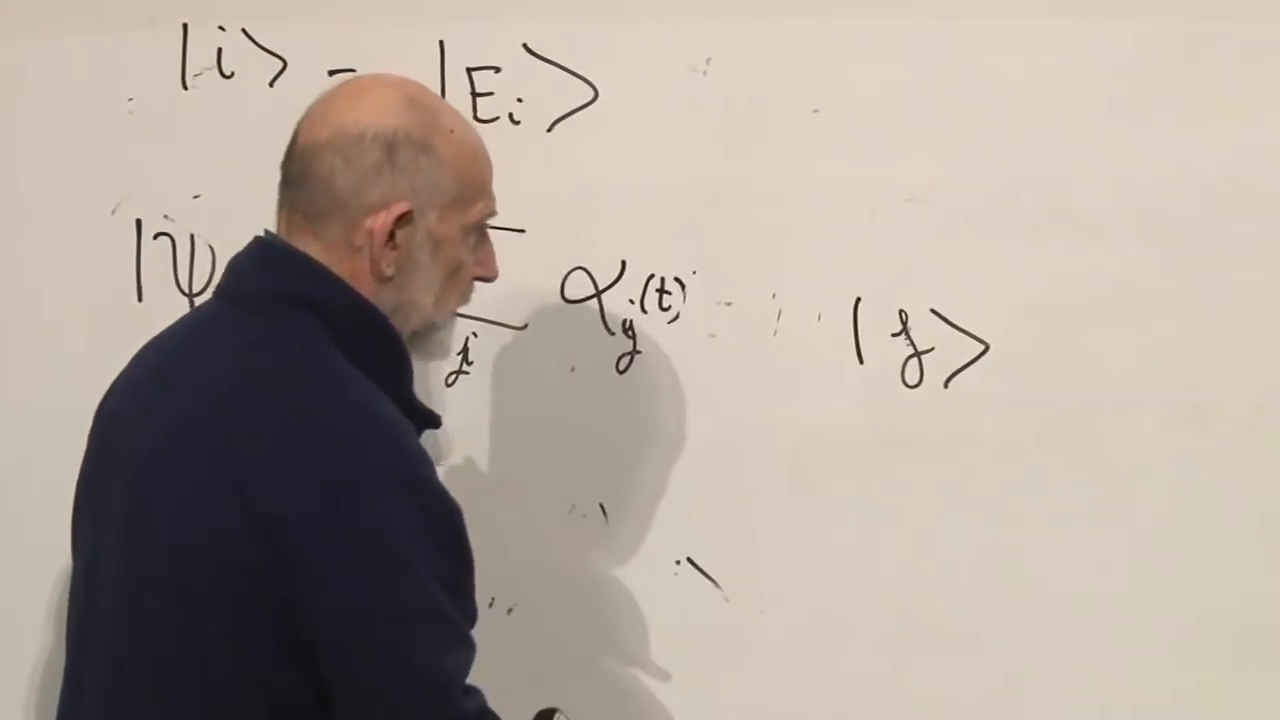
\includegraphics[width=0.86\textwidth]{lecture_05_figure_05.png}
\caption{將等式兩邊展開以驗證對易子的乘法法則。}
\lectureframe{00:43:10}
\end{figure}

\begin{classroomqa}
\audiencequestion{乘法法則右邊是不是不小心把左邊算了兩次？}
\lecturerresponse{沒有。展開後，\(ABC\)與\(-CAB\)正是所需的兩項。額外插入的兩項是\(-ACB\)與\(+ACB\)，它們恰好互相抵消。看似多出一份的部分，是為了以兩種所需方式整理式子而暫時引入的項。}
\end{classroomqa}

經典卜瓦松括號也具有相同的反對稱性與乘法法則。這種結構上的相似並非偶然。量子與經典的對應關係是
\begin{equation}
\{A,B\}
\quad\longleftrightarrow\quad
\frac{1}{i\hbar}[A,B]
=-\frac{i}{\hbar}[A,B].
\label{eq:l5-poisson-correspondence}
\end{equation}
在\(\hbar=1\)的單位制下，經典方程
\begin{equation}
\frac{dL}{dt}=\{L,H\}
\end{equation}
與方程~\eqref{eq:l5-expectation-motion}形式相同。在一般的宏觀單位制下，\(\hbar\)極小，而在適當的經典極限下，對易子可以忽略。這是確認量子生成元\(H\)對應於經典力學哈密頓量的關鍵檢驗。

因子\(\hbar\)在量綱上不可或缺。卜瓦松括號是對正則共軛座標與動量微分而得；算符對易子則直接由算符乘積構成。普朗克常數提供了兩者量綱之間的換算。

令\(L=H\)。由於任何算符都與自身對易，
\begin{equation}
\frac{d}{dt}\expect{H}
=-i\expect{[H,H]}=0.
\end{equation}
對於此處討論的定常哈密頓量，平均能量守恆。關於完整能量分布還能提出更強的陳述，但此處只需要平均值。

\begin{classroomqa}
\audiencequestion{這些方程中的\(L\)是什麼？它是角動量嗎？}
\lecturerresponse{此處的\(L\)是一般的厄米線性算符，也就是任意可觀測量。它可以是自旋分量、位置，甚至是\(H\)本身。這個字母取自「\emph{線性算符}」，除非另有說明，不應把它解讀為角動量。}
\end{classroomqa}

\begin{classroomqa}
\audiencequestion{因子\(i\)為什麼不會使實數期望值的導數變成虛數？}
\lecturerresponse{兩個厄米算符的對易子是反厄米算符，因此它的期望值是虛數。下方的泡利矩陣計算會具體顯示這一點：它們的對易子含有明確的因子\(2i\)，會與運動方程中的\(-i\)互相抵消。}
\end{classroomqa}

\section{在能量基底中求解Schr\"odinger方程}

假設能量本徵值問題已經求解。將任意狀態展開在固定的能量基底中：
\begin{equation}
\ket{\psi(t)}=\sum_j\alpha_j(t)\ket{E_j}.
\label{eq:l5-energy-expansion}
\end{equation}
在這種描述中，基底向量保持不變；所有時間依賴性都包含在係數中。將方程~\eqref{eq:l5-energy-expansion}代入方程~\eqref{eq:l5-schrodinger}，得到
\begin{align}
\sum_j\dot\alpha_j(t)\ket{E_j}
&=-i\sum_j\alpha_j(t)H\ket{E_j}\\
&=-i\sum_j E_j\alpha_j(t)\ket{E_j}.
\end{align}
由於基底展開具有唯一性，對每個固定的\(j\)，都有
\begin{equation}
\dot\alpha_j(t)=-iE_j\alpha_j(t),
\qquad\text{no sum on \(j\)}.
\end{equation}
其解為
\begin{equation}
\alpha_j(t)=\alpha_j(0)e^{-iE_jt}.
\label{eq:l5-energy-phase}
\end{equation}

\begin{figure}[htbp]
\centering
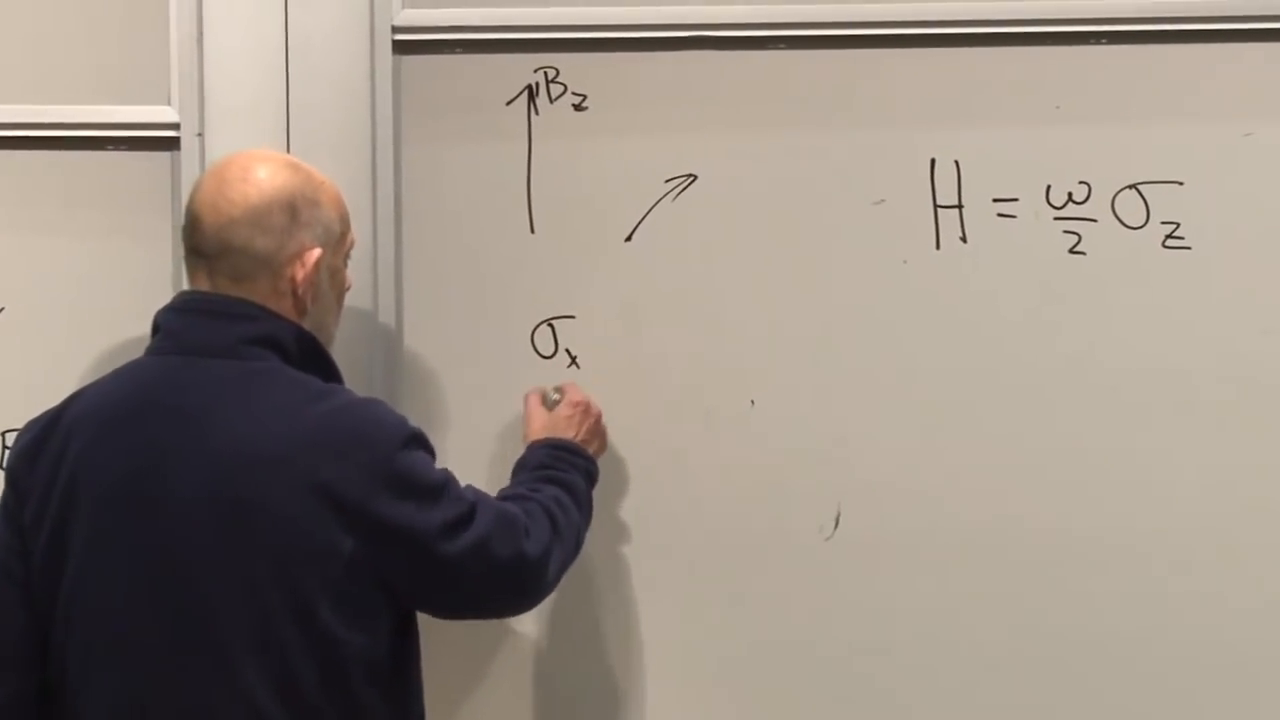
\includegraphics[width=0.86\textwidth]{lecture_05_figure_06.png}
\caption{每個能量基底係數各自滿足一個指數相位方程。}
\lectureframe{01:03:25}
\end{figure}

因此，通解為
\begin{equation}
\ket{\psi(t)}
=\sum_j\alpha_j(0)e^{-iE_jt}\ket{E_j}.
\label{eq:l5-general-solution}
\end{equation}
恢復單位後，\(E_jt\)要改為\(E_jt/\hbar\)。每個係數的大小都保持不變：
\begin{equation}
|\alpha_j(t)|=|\alpha_j(0)|.
\end{equation}
時間演化會改變相對相位。單一能量本徵態只會得到一個共同相位，因此其測量機率不隨時間改變。

現在可以明確寫出\(L\)的期望值。定義它在能量基底中的矩陣元素：
\begin{equation}
L_{kj}=\bra{E_k}L\ket{E_j}.
\end{equation}
於是
\begin{align}
\expect{L}(t)
&=\sum_{k,j}
\alpha_k^*(0)\alpha_j(0)
e^{i(E_k-E_j)t}
L_{kj}.
\label{eq:l5-heisenberg-matrix}
\end{align}

\begin{figure}[htbp]
\centering
\includegraphics[width=0.86\textwidth]{lecture_05_figure_07.png}
\caption{能量基底中的矩陣公式：每個矩陣元素都帶有一個躍遷頻率相位。}
\lectureframe{01:10:45}
\end{figure}

對角項\(k=j\)是常數。非對角矩陣元素則以能量差\(E_k-E_j\)振盪。依照此處的歷史敘述，海森堡在現代態向量推導出現之前，就已認識到這種矩陣結構；後來狄拉克的記號讓它的意義變得清楚。

\begin{classroomqa}
\audiencequestion{\(\alpha_j\)係數的大小會保持不變嗎？}
\lecturerresponse{會。每個係數都乘上一個大小為一的複數相位。改變的只有相對相位，而正是這些相位讓包含非對角矩陣元素的期望值隨時間變化。}
\end{classroomqa}

\begin{classroomqa}
\audiencequestion{Schr\"odinger方程應該使用偏導數還是全導數？}
\lecturerresponse{此處使用的抽象狀態\(\ket{\psi(t)}\)只有時間這一個明示的變數，因此兩種記號表達的內容相同。稍後，像\(\psi(x,t)\)這樣的波函數會同時依賴位置與時間，屆時使用偏導數記號就很自然。}
\end{classroomqa}

\begin{classroomqa}
\audiencequestion{正交性的保持只是經驗假設嗎？}
\lecturerresponse{實驗支持這項原理，但它也格外嚴格。若試圖任意改變酉量子力學，往往會破壞正定性或機率守恆、因果局域性，或複合系統的一致處理。David Finkelstein 將可形變理論比喻為塑性流動，將剛性理論比喻為脆性破裂。量子力學在這個意義上是脆性的：任意微小的改動通常都無法導向一個相近且自洽的理論。}
\end{classroomqa}

\begin{classroomqa}
\audiencequestion{能量本徵值\(E_j\)為什麼是實數？}
\lecturerresponse{酉性表示無窮小生成元\(H\)是厄米算符，而厄米算符的本徵值全為實數。因此，整個推論鏈是：保持正交性、酉性、\(H\)的厄米性，以及能譜為實數。}
\end{classroomqa}

\section{磁場中的自旋}

單一自旋應該配上什麼哈密頓量？孤立自旋若處於其他方面皆空無一物的空間，就沒有特別優先的方向，因此其哈密頓量正比於單位算符，不會造成可觀測的運動。磁場則提供了交互作用能與一條軸向。

令磁場沿\(z\)方向。帶電且具有自旋的粒子帶有磁矩；熟知的偶極能量與磁矩沿磁場方向的分量成正比。將磁場強度、磁矩、正負號慣例及\(\hbar\)吸收到常數\(\omega\)中：
\begin{equation}
H=\frac{\omega}{2}\sigma_z.
\label{eq:l5-z-hamiltonian}
\end{equation}
採用\(1/2\)這個因子很方便，因為泡利對易子含有因子\(2\)。

使用經典箭頭的圖像時必須謹慎。量子自旋的\(x\)、\(y\)與\(z\)分量不可能同時具有確定值，因此普通的箭頭無法同時代表它的所有性質。有用的三維物件是期望值向量，而不是二分量的態向量本身。

\subsection{泡利對易子}

使用以下矩陣表示：
\begin{equation}
\begin{aligned}
\sigma_x&=
\begin{pmatrix}0&1\\1&0\end{pmatrix},\\[0.4em]
\sigma_y&=
\begin{pmatrix}0&-i\\i&0\end{pmatrix},\\[0.4em]
\sigma_z&=
\begin{pmatrix}1&0\\0&-1\end{pmatrix}.
\end{aligned}
\end{equation}
例如，
\begin{align}
[\sigma_z,\sigma_x]
&=
\begin{pmatrix}1&0\\0&-1\end{pmatrix}
\begin{pmatrix}0&1\\1&0\end{pmatrix}
-
\begin{pmatrix}0&1\\1&0\end{pmatrix}
\begin{pmatrix}1&0\\0&-1\end{pmatrix}\\
&=
\begin{pmatrix}0&1\\-1&0\end{pmatrix}
-
\begin{pmatrix}0&-1\\1&0\end{pmatrix}\\
&=2
\begin{pmatrix}0&1\\-1&0\end{pmatrix}
=2i\sigma_y.
\end{align}
循環關係為
\begin{equation}
\begin{aligned}
[\sigma_z,\sigma_x]&=2i\sigma_y,\\
[\sigma_x,\sigma_y]&=2i\sigma_z,\\
[\sigma_y,\sigma_z]&=2i\sigma_x.
\end{aligned}
\label{eq:l5-pauli-commutators}
\end{equation}
交換任一對易子中的兩個項目，符號都會反轉。

\begin{figure}[htbp]
\centering
\includegraphics[width=0.86\textwidth]{lecture_05_figure_08.png}
\caption{三個泡利對易子循環地由泡利矩陣本身構成封閉關係。}
\lectureframe{01:33:30}
\end{figure}

這些關係與角動量的經典卜瓦松括號具有相同的循環結構。它們也只由原來的三個算符構成封閉關係，因此運動方程特別簡單。

\begin{classroomqa}
\audiencequestion{一定要用 bra-ket 括號來計算對易子嗎？}
\lecturerresponse{不用。算符相乘對應於矩陣相乘，因此直接計算\(2\times2\)矩陣很方便。也可以依序將算符作用在自旋向上與向下的基底態上，結果相同。}
\end{classroomqa}

\subsection{期望值的進動}

將方程~\eqref{eq:l5-expectation-motion}與方程~\eqref{eq:l5-z-hamiltonian}中的哈密頓量一併代入：
\begin{align}
\frac{d}{dt}\expect{\sigma_x}
&=-i\frac{\omega}{2}\expect{[\sigma_x,\sigma_z]}
=-\omega\expect{\sigma_y},\\
\frac{d}{dt}\expect{\sigma_y}
&=-i\frac{\omega}{2}\expect{[\sigma_y,\sigma_z]}
=+\omega\expect{\sigma_x},\\
\frac{d}{dt}\expect{\sigma_z}
&=-i\frac{\omega}{2}\expect{[\sigma_z,\sigma_z]}
=0.
\label{eq:l5-spin-motion}
\end{align}

\begin{figure}[htbp]
\centering
\begin{minipage}[c]{0.62\textwidth}
\centering
\includegraphics[width=\textwidth]{lecture_05_figure_09.png}
\end{minipage}\hfill
\begin{minipage}[c]{0.31\textwidth}
\centering
\begin{tikzpicture}[scale=0.78,>=Latex]
  \draw[->,thick] (0,0) -- (0,3.0) node[above] {\(z\parallel\bm B\)};
  \draw[dashed] (0,1.8) ellipse (1.45 and 0.42);
  \draw[->,very thick] (0,0) -- (1.05,1.8)
    node[right] {\(\expect{\bm\sigma}\)};
  \draw[->,thick] (1.38,1.67)
    arc[start angle=-12,end angle=245,x radius=1.45,y radius=0.42];
\end{tikzpicture}
\end{minipage}
\caption{黑板上的方程及其幾何結果：橫向期望值旋轉，平行於磁場的分量則保持不變。箭頭表示三個期望值，而非某個隱藏的經典自旋。}
\lectureframe{01:35:28}
\end{figure}

前兩個方程描述橫向平面上的圓周運動：
\begin{align}
\expect{\sigma_x}(t)
&=\expect{\sigma_x}(0)\cos\omega t
-\expect{\sigma_y}(0)\sin\omega t,\\
\expect{\sigma_y}(t)
&=\expect{\sigma_x}(0)\sin\omega t
+\expect{\sigma_y}(0)\cos\omega t.
\end{align}
另一方面，\(\expect{\sigma_z}\)保持不變。因此，期望值向量會以角頻率\(\omega\)繞著磁場軸進動。

在這個Schr\"odinger表象的計算中，算符是固定的矩陣。改變的是狀態，因此隨熟悉的陀螺運動變化的是平均值。

\begin{classroomqa}
\audiencequestion{二維的態空間怎麼會呈現三維進動？}
\lecturerresponse{態向量有兩個複數分量，差異只在規範化與整體相位。圖中實空間的向量則是\(\bigl(\expect{\sigma_x},\expect{\sigma_y},\expect{\sigma_z}\bigr)\)。這些期望值由狀態決定，構成布洛赫向量圖像，但它們並不是態向量本身。}
\end{classroomqa}

\section{最一般的單一自旋哈密頓量}

每個厄米\(2\times2\)矩陣都可以展開為
\begin{equation}
H=aI+b_x\sigma_x+b_y\sigma_y+b_z\sigma_z,
\end{equation}
其中係數皆為實數。單位算符項只會改變整體相位。其餘三個係數可視為某個向量的分量。令其大小為\(\omega/2\)，方向由單位向量\(\bm n\)表示，則非平凡的哈密頓量可寫為
\begin{equation}
H=\frac{\omega}{2}\,\bm\sigma\cdot\bm n,
\qquad
\bm\sigma\cdot\bm n
=n_x\sigma_x+n_y\sigma_y+n_z\sigma_z.
\label{eq:l5-general-spin-h}
\end{equation}
若\(\bm B=B\bm n\)，則\(\bm n\)表示磁場方向，而\(\omega\)則包含磁耦合在內的場強大小。記錄方向的是\(\bm n\)，不是\(\omega\)。

運動方程可簡潔地寫成
\begin{equation}
\frac{d}{dt}\expect{\bm\sigma}
=\omega\,\bm n\times\expect{\bm\sigma}.
\end{equation}
沿著\(\bm n\)的分量與\(H\)對易，因此保持不變；垂直分量則繞\(\bm n\)進動。

\begin{classroomqa}
\audiencequestion{為什麼哈密頓量應該採用這種形式？}
\lecturerresponse{獨立的厄米\(2\times2\)矩陣只有四個：\(I,\sigma_x,\sigma_y,\sigma_z\)。單位矩陣不會造成可觀測的單一自旋運動，因此任何非平凡且與時間無關的單一自旋哈密頓量，都是三個泡利矩陣的實係數線性組合。磁場則將這三個係數整合成大小與方向。}
\end{classroomqa}

\begin{classroomqa}
\audiencequestion{\(\omega\)究竟代表什麼？}
\lecturerresponse{它是與磁場大小和磁矩乘積成正比的純量，慣用常數已吸收其中。它同時決定進動頻率與能階分裂。單位向量\(\bm n\)表示磁場方向。}
\end{classroomqa}

\subsection{兩個能階}

將方程~\eqref{eq:l5-general-spin-h}寫成矩陣形式，得到
\begin{equation}
\bm\sigma\cdot\bm n
=
\begin{pmatrix}
n_z & n_x-in_y\\
n_x+in_y & -n_z
\end{pmatrix}.
\end{equation}
令其本徵值為\(\lambda_1,\lambda_2\)。矩陣的跡為零：
\begin{equation}
\lambda_1+\lambda_2=0.
\end{equation}
對單位向量\(n_x^2+n_y^2+n_z^2=1\)而言，其行列式為
\begin{align}
\lambda_1\lambda_2
&=\det(\bm\sigma\cdot\bm n)\\
&=-n_z^2-(n_x-in_y)(n_x+in_y)\\
&=-(n_x^2+n_y^2+n_z^2)\\
&=-1.
\end{align}
因此，兩個本徵值為
\begin{equation}
\lambda_\pm=\pm1.
\end{equation}

\begin{figure}[htbp]
\centering
\includegraphics[width=0.86\textwidth]{lecture_05_figure_10.png}
\caption{由跡與行列式可得，\(\bm\sigma\cdot\bm n\)的本徵值為\(+1\)與\(-1\)。}
\lectureframe{01:59:20}
\end{figure}

因此，
\begin{equation}
E_\pm=\pm\frac{\omega}{2},
\qquad
\Delta E=E_+-E_-=\omega.
\label{eq:l5-spin-gap}
\end{equation}
磁場方向會改變能量本徵向量，但不會改變這兩個本徵值。

\begin{classroomqa}
\audiencequestion{光子發射和這些能階有什麼關係？}
\lecturerresponse{若將輻射場也納入考慮，較高的自旋能階可以衰變至較低能階，並發射能量為\(\Delta E=\omega\)的光子；此處採用\(\hbar=1\)的慣例。接著，自旋會在沿磁場軸的兩個相反取向之間翻轉。進動計算忽略了這項微弱的輻射耦合，因此自旋可能進動許多次之後才發射光子。}
\end{classroomqa}

\begin{classroomqa}
\audiencequestion{為什麼磁場被視為數值，而不是量子算符？}
\lecturerresponse{暫且將磁體視為質量很大的經典儀器，其漲落與反沖都可忽略。完整的描述會將磁體納入更大的量子系統。當儀器具有許多自由度，而且相關變數的漲落小到電子無法顯著改變它們時，實務上將系統與儀器分開處理便有其合理性。}
\end{classroomqa}

\begin{classroomqa}
\audiencequestion{平滑的進動方程描述每一次個別實驗嗎？}
\lecturerresponse{這些方程描述的是期望值，也就是對以相同方式製備的多次實驗取平均。個別測量仍具有機率性。重複取樣的結果通常會接近理論平均值，但機率論不保證每個有限序列都恰好得到特定結果；就像擲一百萬次硬幣，正面也不一定剛好占一半。}
\end{classroomqa}

\begin{classroomqa}
\audiencequestion{如果自旋指向側面，躍遷會發射半個光子嗎？}
\lecturerresponse{不會。側向的自旋態是兩個能量本徵態的疊加。在對稱情況下，它處於較高能階與較低能階的機率各為一半。因此，它可能發射一個能量為\(\omega\)的完整光子，也可能完全不發射。平均發射能量可以是\(\omega/2\)，但沒有任何單一光子只帶有一半的能階差。}
\end{classroomqa}

單一自旋所有非平凡且與時間無關的動力學，到此已全部討論完畢。最初揭示不確定性的同一套代數，也生成了自旋的運動：彼此不對易的泡利矩陣使哈密頓量導致進動，而與哈密頓量對易的分量則保持守恆。接下來的複雜化，不是改用另一個單一自旋哈密頓量，而是擴大狀態空間，讓獨立系統得以組合並形成糾纏。
